\subsection{Experimental Method} %Measurement of $A_{zz}$ }

As in the case for E12-13-011, the measured double differential cross section for a spin-1 target characterized by a vector polarization $P_{z}$ and tensor polarization
$P_{zz}$ is expressed as,
\begin{equation}
\frac{d^2\sigma_p}{d\Omega dE'}=\frac{d^2\sigma_u}{d\Omega dE'}\left(1-P_zP_BA_1+\frac{1}{2}P_{zz}A_{zz}\right),
\label{eq:one}
\end{equation}
where, $\sigma_p$ ($\sigma_u$) is the polarized (unpolarized) cross section, $P_B$ is the incident electron beam polarization, and $A_1$ ($A_{zz}$) is the
vector (tensor) asymmetry of the virtual-photon deuteron cross section.  This allows us to write
the polarized tensor asymmetry with $0<P_{zz}\leq 1$ using an unpolarized electron beam as
\begin{eqnarray}
\label{Azz}
A_{zz} = \frac{2}{P_{zz}}\left(\frac{\sigma_p - \sigma_u}{\sigma_u}\right).
\end{eqnarray}
The tensor polarization is given by 
\begin{equation}
P_{zz}=\frac{n_+-2n_0+n_-}{n_++n_-+n_0},
\end{equation}
where $n_m$ represents the population in the $m_z=+1$,~$-1$,~or $0$ state.

Eq. \ref{Azz} reveals that the asymmetry $A_{zz}$ compares two different cross sections measured under different polarization conditions of the target: positively tensor polarized and unpolarized.  
To obtain the relative cross section measurement in the same configuration, the same target cup and material will be used at alternating polarization states (polarized vs. unpolarized),  and the magnetic field providing the quantization axis will be oriented along the beamline at all times.
This field will always be held at the same value, regardless of the target material polarization state. 
This process, identical to that used for the E12-13-011 $b_1$ measurement, ensures that the acceptance remains consistent within the stability (10$^{-4}$) of the super conducting magnet.  


Since many of the factors involved in the cross sections cancel in
the ratio, Eq. \ref{Azz} can be expressed in terms 
of the charge normalized, efficiency corrected numbers of tensor polarized ($N_p$) and unpolarized ($N_u$) counts, 
\begin{eqnarray} \label{3}
A_{zz}&=&\frac{2}{fP_{zz}}\left(\frac{N_p - N_u}{N_u}\right) .
\end{eqnarray}

The dilution factor $f$ corrects for the presence of unpolarized nuclei in the target and is defined by
\begin{equation}
f=\frac{N_D\sigma_D}{N_N\sigma_N+N_D\sigma_D+\sum\limits_{A} N_A\sigma_A},
\end{equation}
where $N_D$ is the number of deuterium nuclei in the target and $\sigma_D$ is the corresponding inclusive double differential scattering cross 
section, $N_N$ is the nitrogen number of scattered nuclei with cross section $\sigma_N$, and $N_A$ is the number of other scattering nuclei of mass number $A$ with cross section $\sigma_A$. As has been noted in previous work~\cite{Frankfurt:1988nt}, the dilution factor at high $x$ drops off considerably until the SRC plateau region, as shown in Fig.~\ref{fdil}. By using a high-luminosity solid target and a low scattering angle $\theta_{e'}$, this effect will be counteracted.

\begin{figure}
\begin{center}
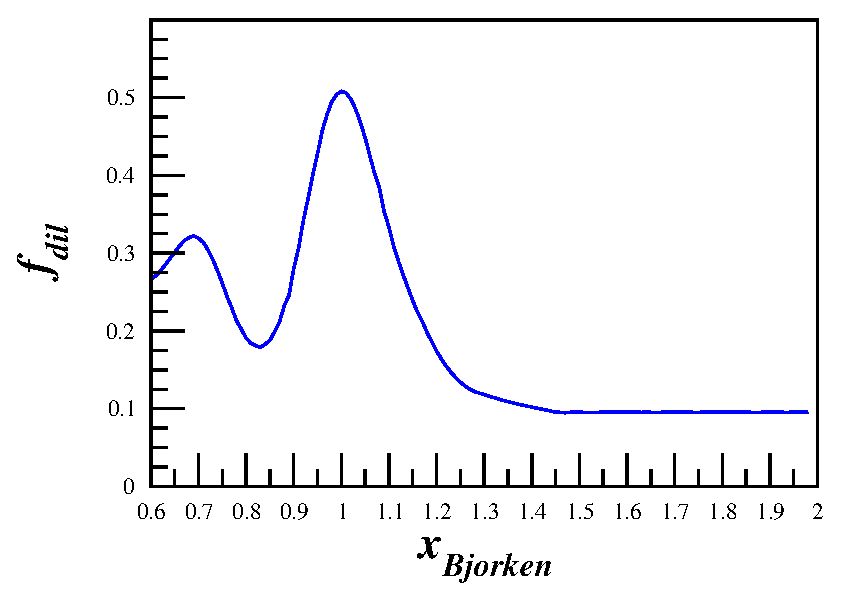
\includegraphics[width=0.45\textwidth]{figs/fdil_q2_15.eps}
\caption{\label{fdil}The estimated dilution factor, in this case at $Q^2=1.5 \mathrm{~(GeV}/c)^2$, is expected to drop off at high $x$ until it reaches the SRC plateau region. This effect will be counteracted by using a high-luminosity solid target.}
\end{center}
\end{figure}

The dilution factor can be written in terms of the relative volume ratio of ND$_3$ to LHe in the target cell, otherwise known as the packing fraction $p_f$.  
In our case of a cylindrical target cell oriented along the magnetic field,the packing fraction is exactly equivalent to the percentage of the cell length filled with ND$_3$.  
%The dilution factor is discussed in further detail in Sec. \ref{dil}.

If the time is evenly split between scattering off of polarized and unpolarized ND$_3$, the time necessary to achieve the desired precision $\delta A$ is:
\begin{equation}
T=\frac{N_p}{R_p}+\frac{N_u}{R_u}=\frac{8}{f^2P_{zz}^2}\left(\frac{R_p(R_u+R_p)}{R_u^3}\right)\frac{1}{\delta A_{zz}^2}
\end{equation} 
where $R_{p(u)}$ is the polarized (unpolarized) rate and $N_{p(u)}$ is the total estimated 
number of polarized (unpolarized) counts to achieve the uncertainty $\delta A_{zz}$.  

%See Sec.~\ref{stat} for full details of the statistical uncertainty.

\subsubsection{Statistical Uncertainty}
\label{stat}
To investigate the statistical uncertainty we start with the equation for $A_{zz}$ using
measured counts for polarized data ($N_p$) and unpolarized data ($N_u$), 
\begin{equation}
A_{zz}=\frac{2}{fP_{zz}}\left(\frac{N_p}{N_u}-1\right).
\end{equation}
The statistical error with respect to counts is then
\begin{equation}
\delta A_{zz}=\frac{2}{fP_{zz}}\sqrt{\left(\frac{\delta N_p}{N_u}\right)^2+\left(\frac{N_p\delta N_u}{N_u^2}\right)^2}.
\end{equation}
For $\delta N_{p(u)}=\sqrt{N_{p(u)}}$, the uncertainty becomes
\begin{equation}
\delta A_{zz}=\frac{2}{fP_{zz}}\sqrt{\frac{N_p(N_u + N_p)}{N_u^3}},
\end{equation}
which can't be simplified further due to the large expected asymmetry.


\subsubsection{Systematic Uncertainty}% in $A_{zz}$ }
\begin{table}
\begin{center}
\begin{tabular}{l|c}\hline\hline
Source                         & Systematic \\
\hline
Polarimetry                  &   12\%   \\
Dilution/Packing fraction    &   6.5\%   \\
Trigger/Tracking efficiency  & 1.0\% \\
Acceptance  		     & 0.5\% \\
Charge Determination           &  1.0\%  \\
Detector resolution and efficiency & 1.0\% \\
\hline
Total  &  14\%   \\
\hline
\end{tabular}
\caption{\label{error1}Estimates of the scale dependent contributions to the systematic error of $A_{zz}$.}
\end{center}
\end{table}

Table \ref{error1} shows a list of the scale dependent uncertainties contributing to the systematic error in $A_{zz}$.
With careful uncertainty minimization in polarization the relative error in $P$ can be less than or equal to 3.9\%, as demonstrated in the recent E08-027/E08-007 experiment~\cite{NIMDUST} and nearly as good for the deuteron using multiple techniques to measure the NMR signal as discussed in ~\cite{PTSTDUST}.  With the use of a positive tensor enhanced target it has been projected to be able to achieve a relative error in $P_{zz}$ better than 12\% ~\cite{PTSTDUST}.  The uncertainty from the dilution in the polarized target is estimated to be
about 6\% over the range of kinematics points of interest.  We consider separately the uncertainty in the packing fraction of the ammonia target contributes at a level of less than 3\%.

Charge calibration and detector efficiencies are expected to be known better to 1\%, but the impact of time-dependent drifts in these quantities must be carefully controlled.

\subsubsection*{Time dependent factors}
Eq.~\ref{3} involves the ratio of counts, which leads to cancellation of several first order systematic effects.  However, the fact that the two data sets will not be taken simultaneously leads to a sensitivity to time dependent variations which will need to be carefully monitored and suppressed.
%
To investigate the systematic differences in the time dependent components of the integrated counts, we need to consider the effects from calibration, efficiency, acceptance, and luminosity between the two polarization states.

Fluctuations in luminosity due to target density variation can easily be kept to a minimum by keeping the material beads at the same temperature for both polarization states by control of the microwave and the LHe evaporation.  The He vapor pressure reading can give accuracy of material temperature changes at the level of $\sim$0.1\%.
Beam rastering can also be controlled to a high degree.

The beam charge asymmetries between two helicity states using the luminosity monitors for experiment
E06-010 has been shown to be at the level of $4 \times 10^{-5}$ with a width of $2 \times 10^{-4}$.
An additional estimate on the change in the BCM calibration constant is seen in
experiment E08-027 resulting in a absolute deviation of $2 \times 10^{-4}$ over the course of six
days. We expect to be able to minimize long term drifts by careful thermal isolation of
the BCMs, however resulting trends will be studied and corrections implemented.

The acceptance of each cup can only change as a function of time if the magnetic field changes.  
The capacity to set, reset, and hold the target superconducting magnet to a desired holding field causes a field uncertainty of only $\delta B /B=0.01\%$. 
This implies that, like the cup length $l$, the acceptance ${\cal A}$ for each polarization state is the same.

In order to look at the effect on $A_{zz}$ due to drifts in beam current monitor calibration and detector efficiency, we rewrite Eq.~\ref{3} explicitly in terms of the raw measured counts $N_p^c$ and $N_u^c$,
\begin{eqnarray} \label{3c}
\nonumber
A_{zz}&=&\frac{2}{fP_{zz}}\left(\frac{N^c_p}{N^c_u}-1\right) \\
      &=&\frac{2}{fP_{zz}}\left(\frac{Q\varepsilon l \cal{A}}{Q_1\varepsilon_1 l \cal{A}}\frac{N_p}{N_u}-1\right)
\end{eqnarray}
where $Q$ represents the accumulated charge, and $\varepsilon$ is the detector efficiency. The target length $l$ and acceptance $\cal{A}$ are identical in both states to first order.

We can then express $Q_1$ as the change in beam current measurement calibration that occurs in
the time it takes to collect data in one polarization state before switching to another, such that $Q_1=Q(1-dQ)$.
In this notation $dQ$ is a dimensionless ratio of changes in different polarization states.  A similar representation
is used for drifts in detector efficiency leading to,
\begin{equation}
A_{zz}=\frac{2}{fP_{zz}}\left(\frac{N_pQ(1-dQ)\varepsilon(1-d\varepsilon)}{N_u Q\varepsilon}-1\right).
\end{equation}
which simplifies to,
\begin{equation}
A_{zz}=\frac{2}{fP_{zz}}\left(\frac{N_p}{N_u}(1-dQ-d\varepsilon+dQd\varepsilon)-1\right).
\end{equation}

For estimates of the $dQ$ and $d\varepsilon$ we turn to previous experimental
studies.  For HRS detector drift during the JLab transversity experiment E06-010, the detector response was measured such that the normalized yield for same condition over a three month period indicated little change ($<1$\%).
These measurement were then used to show that for short time (20 minutes periods between target spin flip),
the detector drift was estimated to be less than 1\% times the ratio of the time period between target spin flip and three months.
For the present experiment we use the same estimate except for the period between target polarization states used is
$\sim$12 hours leading to an overall drift $d\varepsilon\sim0.01\%$.  A similar approach is used to establish an estimate
for $dQ$ using studies from the data from the E08-027 experiment resulting in $d\varepsilon\sim0.01\%$.

To express $A_{zz}$ in terms of the estimated experimental drifts in efficiency and current measurement we can write,
\begin{equation}
A_{zz}=\frac{2}{fP_{zz}}\left(\frac{N_1}{N}-1\right)\pm\frac{2}{fP_{zz}}d\xi.
\end{equation}
This leads to a contribution to $A_{zz}$ on the order of $1\times10^{-3}$,
\begin{equation}
dA_{zz}^{drift}=\pm\frac{2}{fP_{zz}}d\xi=\pm3.7\times10^{-3}.
\end{equation}
For this estimate we assume only two polarization state changes in a
day. 
If it is possible to increase this rate then the systematic effect in $A_{zz}$ will decrease accordingly.

Naturally detector efficiency can drift for a variety of reasons, for
example including fluctuations in gas quality, HV drift or
drifts in the spectrometers magnetic field.  All of these types of variation as can be realized both
during the experiment though monitoring as well as systematic studies of the data collected.
Checks on the consistency of the cross section data that can be use ensuring the quality of each run will be used in the asymmetry analysis.  Regression can be use to correct for any long term drifts that are of a non-stochastic nature.
Each of these systematic effects can mitigate the systematic uncertainty to $\sim0.001$. 
In the kinematic region proposed here, $A_{zz}$ is expected to be large, on the order of $0.1$ to $1.0$, making any absolute errors on this scale only critical as the data and models pass through the x-axis.  While typical false asymmetries in Hall C of $0.01$ are acceptable for this proposed measurement, we are interested in a strict control of the systematics for further reduction.